\part{Devoluciones de estudiantes}
\label{devoluciones}
Como parte del trabajo incluía una prueba de uso por estudiantes, se decidió compartir la herramienta en las comisiones de Organización de Computadoras
del segundo cuatrimestre del 2020.
Al finalizar la cursada fue enviada una encuesta para conocer las opiniones de los y las estudiantes acerca de la herramienta para poder saber qué tan útil resultó la herramienta y conocer ideas de posibles mejoras.

Los gráficos de los resultados obtenidos en la encuesta se pueden ver a continuación.
\begin{figure}[H]
  \centering
  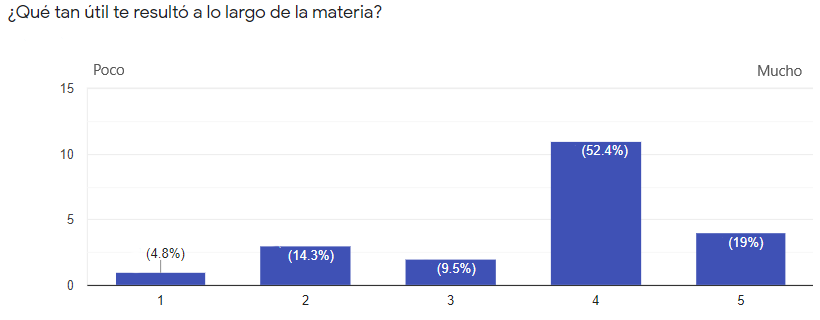
\includegraphics[width=16cm]{figuras/01_encuesta_que_tan_util.png}
\end{figure}

\begin{figure}[H]
  \centering
  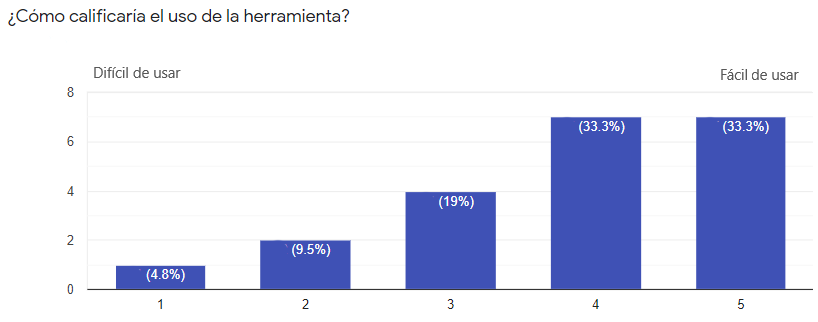
\includegraphics[width=16cm]{figuras/02_encuesta_uso.png}
\end{figure}

\begin{figure}[H]
  \centering
  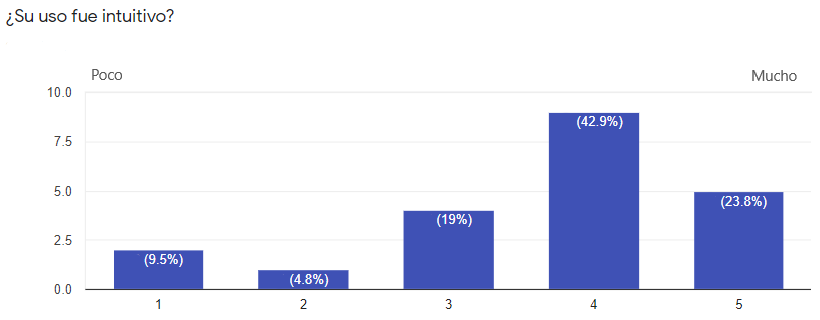
\includegraphics[width=16cm]{figuras/03_encuesta_uso_intuitivo.png}
\end{figure}

\begin{figure}[H]
  \centering
  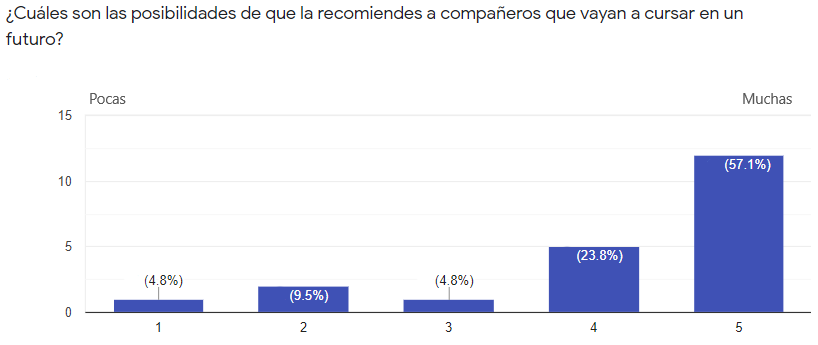
\includegraphics[width=16cm]{figuras/04_encuesta_posibilidad_recomendar.png}
\end{figure}

A pesar de que al comienzo del semestre los alumnos usaron una versión incompleta de QSim Web se puede observar, dado los resultados obtenidos, 
que la herramienta cumplió con su cometido, les fue útil, fácil de usar e intuitiva.

\begin{figure}[H]
  \centering
  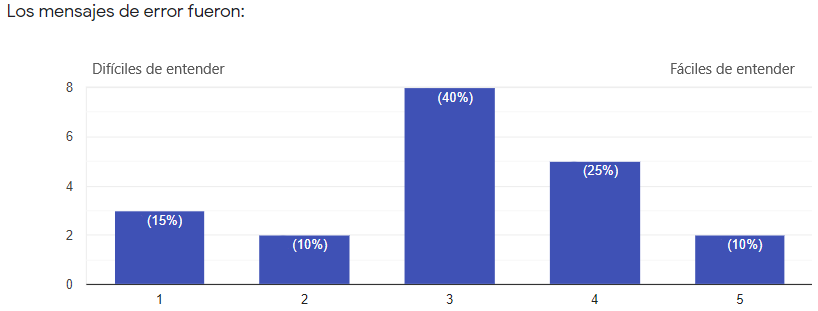
\includegraphics[width=16cm]{figuras/05_encuesta_mensajes_error.png}
\end{figure}
Aquí podemos observar, más allá de que el resultado no fue negativo, que los mensajes de error no fueron suficientemente declarativos.

\begin{figure}[H]
  \centering
  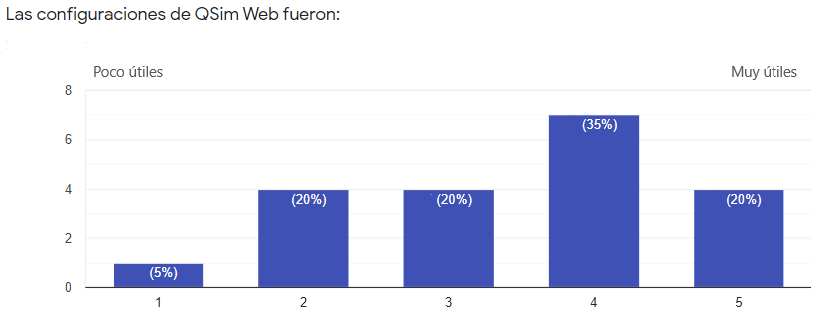
\includegraphics[width=16cm]{figuras/06_encuesta_configuracion.png}
\end{figure}
La configurabilidad de la herramienta nos parece un punto fuerte, pero al estar la mayoría de las funcionalidades habilitadas por defecto, esperábamos que aquí el gráfico tienda a “Poco útiles”. Nos sorprende positivamente que haya sido de utilidad.

\begin{figure}[H]
  \centering
  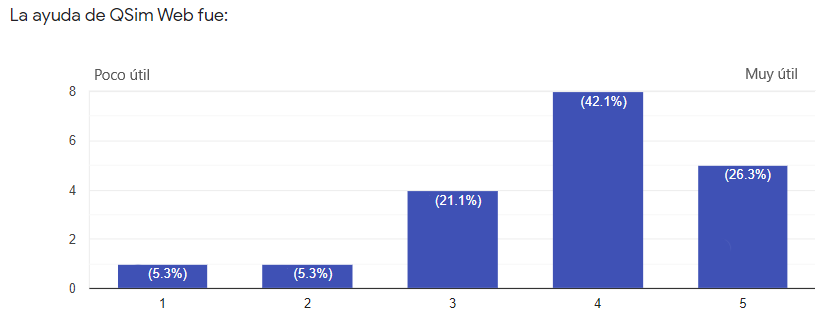
\includegraphics[width=16cm]{figuras/07_encuesta_ayuda.png}
\end{figure}

Además les hemos hecho preguntas donde se podían expresar de forma escrita. 
Estas preguntas apuntaban a conocer su opinión acerca de posibles mejoras de la herramienta, nuevas funcionalidades, funcionalidades que más gustaron y mejoras en la visualización
de resultados.
En general las respuestas fueron positivas y pudimos sacar varias conclusiones e ideas de nuevas funcionalidades para realizar a futuro, como se listarán a continuación.
Muchos comentarios no fueron realizados sobre la última versión de la herramienta, ya que la misma crecía con el pasar del cuatrimestre, y algunas de las funcionalidades pedidas
ya se encontraban implementadas.

Las nuevas funcionalidades son:
\begin{itemize}
  \item Mejorar la sección de ayuda.
  \item Mejorar descripción de errores de sintaxis.
  \item Mejorar resaltado de sintaxis.
  \item Visualización de resultados en Ca2.
  \item Dar la posibilidad de ejecutar instrucciones paso a paso automaticamente con un tiempo de diferencia entre cada una.
  \item Poder detener la ejecución.
  \item Resaltado de la linea de código que se está ejecutando.
  \item Cuando se detecta un error de sintaxis, además de marcarlo dar una posible solución.
  \item Poder modificar valores de registros, memoria y flags mientras se está ejecutando un programa.
\end{itemize}